\subsection{Electrical Power System (EPS)}

The choice of a battery and a power distribution module involve to know the needs
in electricity of our components. Even not having all this data now, we
can make a comparison between some elements performances
\cite{isis_solar_panels}\cite{LMRST-Sat}\cite{Usman}.

\subsubsection{Batteries}

\paragraph{Clyde Space SBAT2-30}

Integrated battery heater with thermostat to maintain battery temperature above 0°C.
(Figure \ref{fig:clyde_space_sbat2})
\begin{itemize}
	\item Capacity at -10°C, 0°C, 20°C and 50°C Voltage max 8.4
	\item Charge current 1875 mA
	\item Dimensions 95.885 x 90.17 x 20.44 mm3
	\item Mass 256g
	\item Price 3550\$ (2640 \euro)
\end{itemize}

\begin{figure}[h]
	\centering
	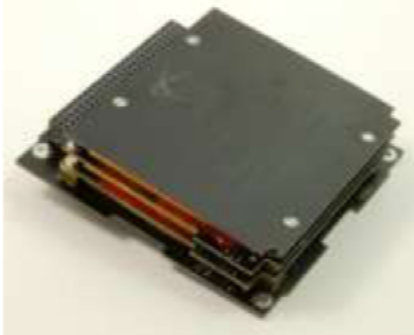
\includegraphics[width=0.5\textwidth]{img/clyde_space_sbat2-30.png}
	\caption{Clyde Space SBAT2-30 batteries}
	\label{fig:clyde_space_sbat2}
\end{figure}

\paragraph{NanoPower BP-4}

\begin{itemize}
	\item Operational temperature: \SI{-1}{\degreeCelsius} to \SI{60}{\degreeCelsius}
	\item Voltage max 8.4 V
	\item Mass: 240g
	\item Dimension: 94 x 88 x 20 mm3
	\item Price 1500 \euro
	\item Capacity: 5200mA
	\item Voltage: 6.0 - 8.4V
	\item Charge current: 2500mA - 5000mA
	\item Discharge current: 0 - 7500mA
\end{itemize}

\begin{figure}[h]
	\centering
	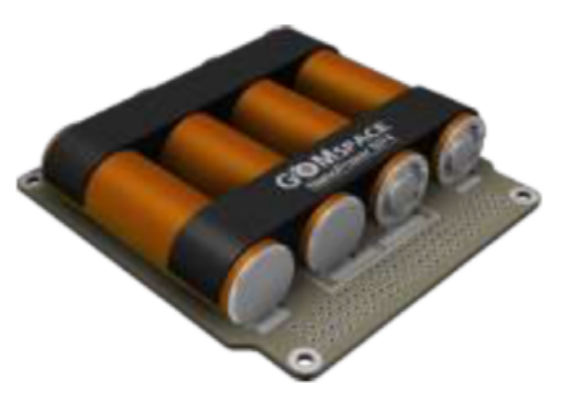
\includegraphics[width=0.5\textwidth]{img/Isispace_nanopower_bp4.png}
	\caption{Isispace NanoPower BP-4 batteries}
	\label{fig:Isispace_nanopower_bp4}
\end{figure}

Those two are more or less equivalent. Their mass, temperatures and maximum voltage
are similar. But the first one got an integrated heater and is more expensive,
because already tested for spatial use.

\subsubsection{Solar Panels}

During its 97 minutes revolution around the earth, our cubesat will be in the
sunlight for approximately 60 minutes. In order to insure its autonomy, we
need some solar panels.

The one we have selected are from Isispace. We need 12W to allow our satellite
to work properly, so we have decided to put 2U panels on each of its 4 faces.
It will gives us 18.4W at its maximum, for a total mass of 400g.

\begin{figure}[h]
	\centering
	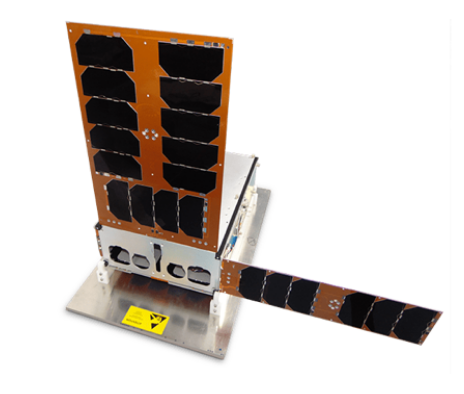
\includegraphics[width=0.5\textwidth]{img/solar_panels.png}
	\caption{Isispace selected solar panels}
	\label{fig:solar_panels}
\end{figure}

\begin{itemize}
	\item Panel Thickness:
	\begin{itemize}
		\item Top/Bottom: 1.8 mm
		\item Side Panel: 2.5 mm
	\end{itemize}
	\item Cover Glass: QioptiQ
	\item Interconnector: Silver plated Kovar
	\item Operating Temperature: \SI{-40}{\degreeCelsius} to \SI{+125}{\degreeCelsius}
	\item Radiation Tolerance: 2 years minimum in LEO
	\item Cell efficiency: 30\%
	\item Price: 500 \euro
\end{itemize}

\subsection{PDM (Power Distribution Module)}

\paragraph{PS (ISISpace) NanoPower P31U Power Supply Performance}

93\% average input converter efficiency
Power consumption: 250 mW
Two regulated power buses: 3.3V@5A and 5V@4A
Lithium-Ion Cells:
\begin{itemize}
	\item Voltage: 3.7V typ. (3.0V min. to 4.2V max.)
	\item Charge current: 1250 mA typ. (2500 mA max.)o Discharge current: 500 mA typ. (3750 mA max.)o Charge temperature: -5 to 45°C
	\item Discharge temperature: -20 to 60°C
	\item Storage temperature: -20 to 20°C
	\item Internal impedance: 70 mOhm
\end{itemize}

Product Properties:
Dimensions: 96mm x 90mm x (16 to 26) mm
PCB material: FR4 Tg180 (HAL finish)
Mass without batteries: 105g
Mass with batteries: 200g
Price: 3300 \euro

But this module only work with the Isispace battery, because it is a lithium-ion one.

\begin{figure}[h]
	\centering
	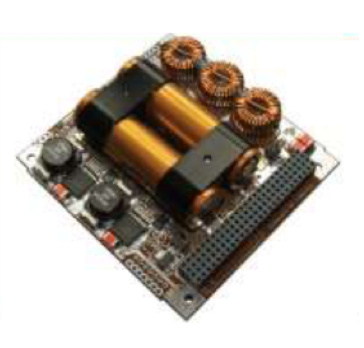
\includegraphics[width=0.5\textwidth]{img/PS_isispace.png}
	\caption{PS (ISISpace) NanoPower P31U Power Supply}
	\label{fig:PS_isispace}
\end{figure}


\paragraph{PS (Clyde Space)}

This module is composed of many battery charge regulators. But as the previous one,
it is only useful with the ClydeSpace battery because it works only with lithium polymer battery.

Performance:

\begin{itemize}
	\item Maximum Available Current: 2.5 A
	\item Power efficiency: 95\%
	\item Max BCR efficiency:
	\item 8W: 90\%
	\item 3W: 79\%
	\item BCR configuration:
	\item 2 x 8W BUCK 1 x 3W SEPIC
\end{itemize}

Product Properties:

\begin{itemize}
	\item Operating Temperature: -40 to +85°C
	\item Radiation Tolerance: 10kRad
	\item Mass: 83g
	\item Height: 15.3 mm
\end{itemize}
Price: 3350 \euro
